% questions.tex —— 2011 年·安徽卷·文科 · 题目内容片段（无答案）
% 由 tools/generate_projects.py 依来源总账自 2011/2011_数学真题_安徽文_试题.md 生成，勿手改（改源 MD 后重跑）
\gkpart{数学}
\begin{gktip}
\textbf{来源说明}：本题面依据固定源 PDF 两页 A3 题面逐栏转录，原卷印刷页码 645–646。固定源不附答案；原页各题与各节均未印分值，记「原页未标」，不补。答案和解析均由本库独立复算。

\textbf{源疑点}：原页除题面外不印分值，也不印参考公式；第 20 题所需的回归系数公式原页未给，本库在解析正文中直接给出最小二乘式并据此计算。第 5 题（A）（C）两选项的值写在括号中以分式排印，按 $\left(\dfrac1a,b\right)$、$\left(\dfrac{10}{a},b+1\right)$ 转录。第 15 题五个结论的编号原页用 ①—⑤，选项不设字母。

\textbf{图形说明}：第 8 题的三视图、第 10 题的函数图象、第 12 题的程序框图、第 19 题的多面体均重绘为 TikZ 矢量图，依原页拓扑重绘，不按比例。原页其余各题无图。
\end{gktip}
\gkpart{一、选择题}
\begin{question}
\gkti{1}设 $\mathrm i$ 是虚数单位，复数 $\dfrac{1+a\mathrm i}{2-\mathrm i}$ 为纯虚数，则实数 $a$ 为\mbox{（　　）}

（A）$2$

（B）$-2$

（C）$-\dfrac12$

（D）$\dfrac12$
\end{question}
\begin{question}
\gkti{2}集合 $U=\{1,2,3,4,5,6\}$，$S=\{1,4,5\}$，$T=\{2,3,4\}$，则 $S\cap(\complement_U T)$ 等于\mbox{（　　）}

（A）$\{1,4,5,6\}$

（B）$\{1,5\}$

（C）$\{4\}$

（D）$\{1,2,3,4,5\}$
\end{question}
\begin{question}
\gkti{3}双曲线 $2x^2-y^2=8$ 的实轴长是\mbox{（　　）}

（A）$2$

（B）$2\sqrt2$

（C）$4$

（D）$4\sqrt2$
\end{question}
\begin{question}
\gkti{4}若直线 $3x+y+a=0$ 过圆 $x^2+y^2+2x-4y=0$ 的圆心，则 $a$ 的值为\mbox{（　　）}

（A）$-1$

（B）$1$

（C）$3$

（D）$-3$
\end{question}
\begin{question}
\gkti{5}若点 $(a,b)$ 在 $y=\lg x$ 图象上，$a\neq1$，则下列点也在此图象上的是\mbox{（　　）}

（A）$\left(\dfrac1a,b\right)$

（B）$(10a,1-b)$

（C）$\left(\dfrac{10}{a},b+1\right)$

（D）$(a^2,2b)$
\end{question}
\begin{question}
\gkti{6}设变量 $x$，$y$ 满足
\nopagebreak[4]
\[
\begin{cases}
x+y\leqslant1,\\
x-y\leqslant1,\\
x\geqslant0,
\end{cases}
\]
则 $x+2y$ 的最大值和最小值分别为\mbox{（　　）}

（A）$1$，$-1$

（B）$2$，$-2$

（C）$1$，$-2$

（D）$2$，$-1$
\end{question}
\begin{question}
\gkti{7}若数列 $\{a_n\}$ 的通项公式是 $a_n=(-1)^n\cdot(3n-2)$，则 $a_1+a_2+\cdots+a_{10}=$\mbox{（　　）}

（A）$15$

（B）$12$

（C）$-12$

（D）$-15$
\Needspace{0.4\textheight}
\end{question}
\begin{question}
\gkti{8}一个空间几何体的三视图如图所示，则该几何体的表面积为\mbox{（　　）}

（A）$48$

（B）$32+8\sqrt{17}$

（C）$48+8\sqrt{17}$

（D）$80$
\nopagebreak[4]
\begin{center}% 2011 年安徽卷文科第 8 题：空间几何体的三视图，求表面积。
% 来源 PDF：普通高考/2011/2011安徽文.pdf，SHA-256 af8382bc2cd47a1d5e08bb622275f77ad100aa4f844b5cfd2fd5cd217de58ffc。
% 原页：第 1 页（A3 三栏）第 1 栏中部，书页码 645。
% 重绘依据：照原页——左上为正（主）视图，边长 4 的正方形，上方标 4、左侧标 4；
%   右上为侧（左）视图，下底 4、上底 2、高 4 的等腰梯形，与主视图上下边齐平；
%   左下为俯视图，边长为 4 的正方形，内部有两条水平线把高分成 1、2、1，
%   左侧以三个双向箭头分别标出 1、2、1；三视图下各标名称，原页不画顶点圆点、不标其他尺寸。
\begin{tikzpicture}[scale=0.55, >=stealth, semithick]
  % 正（主）视图：4 x 4 正方形
  \draw (0,0) -- (4,0) -- (4,4) -- (0,4) -- cycle;
  \draw[<->] (-0.05,4.55) -- (4.05,4.55);
  \node at (2,4.72) {$4$};
  \draw[<->] (-0.55,0) -- (-0.55,4);
  \node at (-0.78,2) {$4$};
  \node at (2,-0.62) {正（主）视图};
  % 侧（左）视图：下底 4、上底 2、高 4 的等腰梯形
  \draw (5.6,0) -- (9.6,0) -- (8.6,4) -- (6.6,4) -- cycle;
  \node at (7.6,-0.62) {侧（左）视图};
  % 俯视图：4 x 4 正方形，两条水平线分成 1、2、1
  \draw (0,-1.4) rectangle (4,-5.4);
  \draw (0,-2.4) -- (4,-2.4);
  \draw (0,-4.4) -- (4,-4.4);
  \draw[<->] (-0.55,-1.4) -- (-0.55,-2.4);
  \node at (-0.78,-1.9) {$1$};
  \draw[<->] (-0.55,-2.4) -- (-0.55,-4.4);
  \node at (-0.78,-3.4) {$2$};
  \draw[<->] (-0.55,-4.4) -- (-0.55,-5.4);
  \node at (-0.78,-4.9) {$1$};
  \node at (2,-6.0) {俯视图};
\end{tikzpicture}
\end{center}
\nopagebreak[4]
\end{question}
\begin{question}
\gkti{9}从正六边形的 6 个顶点中随机选择 4 个顶点，则以它们作为顶点的四边形是矩形的概率等于\mbox{（　　）}

（A）$\dfrac1{10}$

（B）$\dfrac18$

（C）$\dfrac16$

（D）$\dfrac15$
\Needspace{0.4\textheight}
\end{question}
\begin{question}
\gkti{10}函数 $f(x)=ax^n(1-x)^2$ 在区间 $[0,1]$ 上的图象如图所示，则 $n$ 可能是\mbox{（　　）}

（A）$1$

（B）$2$

（C）$3$

（D）$4$
\nopagebreak[4]
\begin{center}% 2011 年安徽卷文科第 10 题：函数 f(x)=a x^n (1-x)^2 在 [0,1] 上的图象，判断 n 的可能值。
% 来源 PDF：普通高考/2011/2011安徽文.pdf，SHA-256 af8382bc2cd47a1d5e08bb622275f77ad100aa4f844b5cfd2fd5cd217de58ffc。
% 原页：第 1 页（A3 三栏）第 2 栏中部，书页码 645。
% 重绘依据：照原页——只画第一象限的直角坐标系，x 轴标 0.5 与 1，y 轴标 0.5（与曲线最高点同高），
%   曲线自原点 O 上升、在 0.5 左侧取最高点、于 x=1 处与 x 轴相切后结束；
%   曲线按原页形状（峰在 0.5 左侧、峰高 0.5、右端水平）取 n=1、a=27/8 的函数绘制，只取形状，不标函数式。
\begin{tikzpicture}[scale=3.1, >=stealth, semithick]
  \draw[->] (-0.15,0) -- (1.26,0) node[right] {$x$};
  \draw[->] (0,-0.08) -- (0,0.66) node[above] {$y$};
  \draw[domain=0:1, samples=240, smooth] plot (\x, {3.375*\x*(1-\x)*(1-\x)});
  \draw (0.5,0) -- (0.5,0.013);
  \node[below=0.04cm] at (0.5,0) {$0.5$};
  \draw (1,0) -- (1,0.013);
  \node[below=0.04cm] at (1,0) {$1$};
  \draw (0,0.5) -- (-0.013,0.5);
  \node[left=0.06cm] at (-0.013,0.5) {$0.5$};
  \node[below left=0.01cm and 0.01cm] at (0,0) {$O$};
\end{tikzpicture}
\end{center}
\nopagebreak[4]
\end{question}
\gkpart{二、填空题}
\begin{question}
\gkti{11}设 $f(x)$ 是定义在 $\mathbf R$ 上的奇函数，当 $x\leqslant0$ 时，$f(x)=2x^2-x$，则 $f(1)=$\gkblank{}。
\Needspace{0.4\textheight}
\end{question}
\begin{question}
\gkti{12}如图所示，程序框图（算法流程图）的输出结果是\gkblank{}。
\nopagebreak[4]
\begin{center}% 2011 年安徽卷文科第 12 题：程序框图（算法流程图），求输出结果。
% 来源 PDF：普通高考/2011/2011安徽文.pdf，SHA-256 af8382bc2cd47a1d5e08bb622275f77ad100aa4f844b5cfd2fd5cd217de58ffc。
% 原页：第 1 页（A3 三栏）第 2 栏下部，书页码 645。
% 重绘依据：照原页——自上而下为「开始」→「T=0,k=0」→「T=T+k」→判断框「T>105?」；
%   判断为「是」时向下经平行四边形「输出 k」到「结束」，为「否」时向右到「k=k+1」，
%   再由 k=k+1 向上、向左回到 T=T+k 上方的流程线（原页在该汇合点画向左的箭头，
%   并在 T=T+k 上方另画一个向下箭头）。原页不标其他文字。
\begin{tikzpicture}[>=stealth, semithick, font=\small]
  % 开始
  \node[draw, rounded corners=0.22cm, minimum width=1.80cm, minimum height=0.65cm] (start) at (0,0) {开始};
  % T=0, k=0
  \node[draw, minimum width=2.90cm, minimum height=0.65cm] (init) at (0,-1.05) {$T=0,\ k=0$};
  \draw[->] (start) -- (init);
  % T=T+k
  \node[draw, minimum width=2.90cm, minimum height=0.65cm] (acc) at (0,-2.80) {$T=T+k$};
  \draw (init.south) -- (0,-2.05);
  \draw[->] (0,-2.05) -- (acc.north);
  % 判断框 T>105?
  \node[draw, diamond, aspect=2.4, minimum width=3.00cm, minimum height=1.25cm] (test) at (0,-4.20) {$T>105$?};
  \draw[->] (acc.south) -- (test.north);
  % 否 分支：k=k+1
  \node[draw, minimum width=1.85cm, minimum height=0.65cm] (inc) at (3.30,-4.20) {$k=k+1$};
  \draw[->] (test.east) -- (inc.west);
  \node[above] at (2.20,-4.15) {否};
  % 回边：k=k+1 向上、向左汇入 T=T+k 上方
  \draw[-] (inc.north) -- (3.30,-2.05);
  \draw[->] (3.30,-2.05) -- (0,-2.05);
  % 输出 k
  \draw (-1.10,-5.90) -- (0.90,-5.90) -- (1.10,-5.20) -- (-0.90,-5.20) -- cycle;
  \node at (0,-5.55) {输出 $k$};
  \draw[->] (test.south) -- (0,-5.18);
  \node[left] at (-0.05,-4.98) {是};
  % 结束
  \node[draw, rounded corners=0.22cm, minimum width=1.80cm, minimum height=0.65cm] (end) at (0,-6.60) {结束};
  \draw[->] (0,-5.92) -- (end.north);
\end{tikzpicture}
\end{center}
\nopagebreak[4]
\end{question}
\begin{question}
\gkti{13}函数 $y=\dfrac{1}{\sqrt{6-x-x^2}}$ 的定义域是\gkblank{}。
\end{question}
\begin{question}
\gkti{14}已知向量 $\boldsymbol a$，$\boldsymbol b$ 满足 $(\boldsymbol a+2\boldsymbol b)\cdot(\boldsymbol a-\boldsymbol b)=-6$，且 $|\boldsymbol a|=1$，$|\boldsymbol b|=2$，则 $\boldsymbol a$ 与 $\boldsymbol b$ 的夹角为\gkblank{}。
\end{question}
\begin{question}
\gkti{15}设 $f(x)=a\sin2x+b\cos2x$，其中 $a$，$b\in\mathbf R$，$ab\neq0$，若 $f(x)\leqslant\left|f\left(\dfrac{\pi}{6}\right)\right|$ 对一切 $x\in\mathbf R$ 恒成立，则
① $f\left(\dfrac{11\pi}{12}\right)=0$；
② $\left|f\left(\dfrac{7\pi}{10}\right)\right|<\left|f\left(\dfrac{\pi}{5}\right)\right|$；
③ $f(x)$ 既不是奇函数，也不是偶函数；
④ $f(x)$ 的单调递增区间是 $\left[k\pi+\dfrac{\pi}{6},k\pi+\dfrac{2\pi}{3}\right]$（$k\in\mathbf Z$）；
⑤ 存在经过点 $(a,b)$ 的直线与函数 $f(x)$ 的图象不相交。
以上结论正确的是\gkblank{}。（写出所有正确结论的编号）
\end{question}
\gkpart{三、解答题}
\begin{question}
\gkti{16}在 $\triangle ABC$ 中，$a$，$b$，$c$ 分别为内角 $A$，$B$，$C$ 所对的边长，$a=\sqrt3$，$b=\sqrt2$，$1+2\cos(B+C)=0$，求边 $BC$ 上的高。
\end{question}
\begin{question}
\gkti{17}设直线 $l_1:y=k_1x+1$，$l_2:y=k_2x-1$，其中实数 $k_1$，$k_2$ 满足 $k_1k_2+2=0$。
（1） 证明 $l_1$ 与 $l_2$ 相交；
（2） 证明 $l_1$ 与 $l_2$ 的交点在椭圆 $2x^2+y^2=1$ 上。
\end{question}
\begin{question}
\gkti{18}设 $f(x)=\dfrac{\mathrm e^x}{1+ax^2}$，其中 $a$ 为正实数。
（1） 当 $a=\dfrac43$ 时，求 $f(x)$ 的极值点；
（2） 若 $f(x)$ 为 $\mathbf R$ 上的单调函数，求 $a$ 的取值范围。
\Needspace{0.4\textheight}
\end{question}
\begin{question}
\gkti{19}如图，$ABEDFC$ 为多面体，平面 $ABED$ 与平面 $ACFD$ 垂直，点 $O$ 在线段 $AD$ 上，$OA=1$，$OD=2$，$\triangle OAB$，$\triangle OAC$，$\triangle ODE$，$\triangle ODF$ 都是正三角形。
（1） 证明直线 $BC\parallel EF$；
（2） 求棱锥 $F-OBED$ 的体积。
\nopagebreak[4]
\begin{center}% 2011 年安徽卷文科第 19 题：多面体 ABEDFC，平面 ABED 与平面 ACFD 垂直，
%   O 在线段 AD 上，OA=1，OD=2，△OAB、△OAC、△ODE、△ODF 都是正三角形。
% 来源 PDF：普通高考/2011/2011安徽文.pdf，SHA-256 af8382bc2cd47a1d5e08bb622275f77ad100aa4f844b5cfd2fd5cd217de58ffc。
% 原页：第 2 页（A3 三栏）第 1 栏中部，书页码 646。
% 重绘依据：照原页——A 在左、D 在右，AD 为被遮挡的虚线；B 在 A 的下方偏右，
%   E 在下方中部、C 在 A 的右上方、F 在正上方偏右；O 在线段 AD 上（图上略偏下标注）。
%   实线：AB、BC、CA、BE、ED、DF、FC、FB、FE；虚线：AD（含 O）、OB、OC、OE、OF。
%   各点位置按原页图形比例摆放，不按真实投影；原页不画顶点圆点。
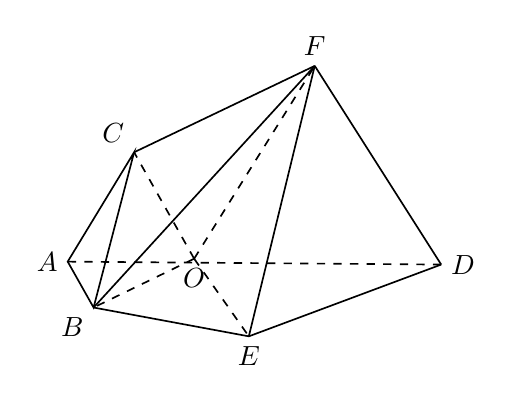
\begin{tikzpicture}[scale=0.62, >=stealth, semithick]
  \coordinate (A) at (0.00,2.20);
  \coordinate (B) at (0.53,1.26);
  \coordinate (C) at (1.36,4.44);
  \coordinate (O) at (2.59,2.26);
  \coordinate (E) at (3.71,0.67);
  \coordinate (D) at (7.65,2.14);
  \coordinate (F) at (5.06,6.21);
  % 可见的棱（实线）
  \draw (A) -- (B) -- (C) -- cycle;
  \draw (B) -- (E) -- (D);
  \draw (F) -- (C);
  \draw (F) -- (B);
  \draw (F) -- (E);
  \draw (F) -- (D);
  % 被遮挡的棱与辅助线（虚线）
  \draw[dashed] (A) -- (D);
  \draw[dashed] (O) -- (B);
  \draw[dashed] (O) -- (C);
  \draw[dashed] (O) -- (E);
  \draw[dashed] (O) -- (F);
  \node at (A) [left]  {$A$};
  \node at (B) [below left] {$B$};
  \node at (C) [above left] {$C$};
  \node at (O) [below] {$O$};
  \node at (D) [right] {$D$};
  \node at (E) [below] {$E$};
  \node at (F) [above] {$F$};
\end{tikzpicture}
\end{center}
\nopagebreak[4]
\end{question}
\begin{question}
\gkti{20}某地最近十年粮食需求量逐年上升，下表是部分统计数据：

\begin{center}
\begin{tabular}{lrrrrr}
\toprule
年份 & 2002 & 2004 & 2006 & 2008 & 2010 \\
\midrule
需求量（万吨） & 236 & 246 & 257 & 276 & 286 \\
\bottomrule
\end{tabular}
\end{center}

（1） 利用所给数据求年需求量与年份之间的回归直线方程 $\hat y=bx+a$；
（2） 利用（1）中所求出的直线方程预测该地 2012 年的粮食需求量。
\end{question}
\begin{question}
\gkti{21}在数 1 和 100 之间插入 $n$ 个实数，使得这 $n+2$ 个数构成递增的等比数列，将这 $n+2$ 个数的乘积记作 $T_n$，再令 $a_n=\lg T_n$，$n\geqslant1$。
（1） 求数列 $\{a_n\}$ 的通项公式；
（2） 设 $b_n=\tan a_n\cdot\tan a_{n+1}$，求数列 $\{b_n\}$ 的前 $n$ 项和 $S_n$。

\end{question}